\documentclass[sigconf,10pt]{acmart}

% *** CITATION PACKAGES ***
%
%\usepackage{cite}
% cite.sty was written by Donald Arseneau
% V1.6 and later of IEEEtran pre-defines the format of the cite.sty package
% \cite{} output to follow that of IEEE. Loading the cite package will
% result in citation numbers being automatically sorted and properly
% "compressed/ranged". e.g., [1], [9], [2], [7], [5], [6] without using
% cite.sty will become [1], [2], [5]--[7], [9] using cite.sty. cite.sty's
% \cite will automatically add leading space, if needed. Use cite.sty's
% noadjust option (cite.sty V3.8 and later) if you want to turn this off.
% cite.sty is already installed on most LaTeX systems. Be sure and use
% version 4.0 (2003-05-27) and later if using hyperref.sty. cite.sty does
% not currently provide for hyperlinked citations.
% The latest version can be obtained at:
% http://www.ctan.org/tex-archive/macros/latex/contrib/cite/
% The documentation is contained in the cite.sty file itself.
%
\usepackage{setspace}
\usepackage{wrapfig}
%\usepackage[usenames, dvipsnames]{color}
\usepackage{balance}
\usepackage{mathtools}
\usepackage{multirow}

%\usepackage[pdftex]{graphicx}
\usepackage{graphicx}
% declare the path(s) where your graphic files are
\graphicspath{{./}{./figs}}
% and their extensions so you won't have to specify these with
% every instance of \includegraphics
\DeclareGraphicsExtensions{.pdf,.jpeg,.png}

% *** SUBFIGURE PACKAGES ***
\usepackage[tight,footnotesize]{subfigure}
% \usepackage{subfigure}
% subfigure.sty was written by Steven Douglas Cochran. This package makes it
% easy to put subfigures in your figures. e.g., "Figure 1a and 1b". For IEEE
% work, it is a good idea to load it with the tight package option to reduce
% the amount of white space around the subfigures. subfigure.sty is already
% installed on most LaTeX systems. The latest version and documentation can
% be obtained at:
% http://www.ctan.org/tex-archive/obsolete/macros/latex/contrib/subfigure/
% subfigure.sty has been superceeded by subfig.sty.

%\usepackage[caption=false]{caption}
%\usepackage[font=footnotesize]{subfig}
% subfig.sty, also written by Steven Douglas Cochran, is the modern
% replacement for subfigure.sty. However, subfig.sty requires and
% automatically loads Axel Sommerfeldt's caption.sty which will override
% IEEEtran.cls handling of captions and this will result in nonIEEE style
% figure/table captions. To prevent this problem, be sure and preload
% caption.sty with its "caption=false" package option. This is will preserve
% IEEEtran.cls handing of captions. Version 1.3 (2005/06/28) and later
% (recommended due to many improvements over 1.2) of subfig.sty supports
% the caption=false option directly:
%\usepackage[caption=false,font=footnotesize]{subfig}
%
% The latest version and documentation can be obtained at:
% http://www.ctan.org/tex-archive/macros/latex/contrib/subfig/
% The latest version and documentation of caption.sty can be obtained at:
% http://www.ctan.org/tex-archive/macros/latex/contrib/caption/

% *** PDF, URL AND HYPERLINK PACKAGES ***
%
\usepackage{url}
% url.sty was written by Donald Arseneau. It provides better support for
% handling and breaking URLs. url.sty is already installed on most LaTeX
% systems. The latest version can be obtained at:
% http://www.ctan.org/tex-archive/macros/latex/contrib/misc/
% Read the url.sty source comments for usage information. Basically,
% \url{my_url_here}.

% *** Do not adjust lengths that control margins, column widths, etc. ***
% *** Do not use packages that alter fonts (such as pslatex).         ***
% There should be no need to do such things with IEEEtran.cls V1.6 and later.
% (Unless specifically asked to do so by the journal or conference you plan
% to submit to, of course. )

\usepackage{draftwatermark}

\newcommand{\assign}[1]{\textcolor{red}{(#1)}}
\newcommand{\todo}[1]{\textcolor{orange}{TODO: #1}}
\newcommand{\fixme}[1]{\textcolor{green}{(#1)}}

%Conference
\acmConference[SC'17]{The International Conference for High Performance Computing, Networking, Storage and Analysis}{November 2017}{Denver, Colorado USA}
\acmYear{2017}
\copyrightyear{2017}

\begin{document}
\title{Towards Total Knowledge of I/O through Integrated Multicomponent Instrumentation}

\begin{abstract}
%%% I had to submit a 150-word abstract to SC, so below is the shortened
%%% version I submitted
%
% As scientific computing becomes more data-intensive and storage hierarchies
% deepen, I/O performance is becoming increasingly critical to productivity in
% HPC.  Instrumentation and analysis tools have long been used to understand
% parallel I/O performance, but analyzing the individual components of I/O
% subsystems in isolation fails to answer how these components interact and
% result in poor I/O performance.
%
% To this end, we have developed a framework for holistic I/O characterization
% that integrates instrumentation from file system servers, applications, file
% system health monitors, and other system resources.  Along with formalized
% periodic regression benchmarking, we then demonstrate this framework's
% portability and unobtrusiveness by deploying it in production on two
% leadership-class computing platforms.  Using data collected during a month
% long study, we provide unique insights into applications' I/O performance
% that are enabled by this approach.  We then extend these findings to provide
% a broader understanding of how application performance varies across
% different file systems and workloads.

I/O efficiency is essential to productivity in scientific computing,
especially as most scientific domains become more data-intensive and
new large-scale computing platforms incorporate more complex storage
hierarchies.  A variety of instrumentation and analysis tools have been
utilized to great effect to help understand and optimize specific aspects of
HPC I/O, such as application access patterns, storage device traffic, and
distributed file system configurations.  However, analyzing individual services in the
I/O ecosystem in isolation fails to provide insight into the most important
questions: how do the I/O components interact, what \emph{combinations}
of optimizations across the stack are most effective, and what are the
underlying causes and effects of I/O performance problems?

In this work we explore the potential for holistic I/O characterization
by combining I/O instrumentation data from multiple sources to obtain
insights that were previously unobtainable. We describe a methodology that
incorporates file system instrumentation, application instrumentation,
health monitoring, and formalized periodic regression benchmarking and demonstrate
the applicability, portability, and unobtrusiveness of this approach by
deploying it in production on two distinct leadership-class computing
platforms.
%
% Based on our month-long study, we demonstrate the utility of our
% methodology through case studies that highlight how holistic I/O
% characterization can improve our understanding of scientific applications'
% I/O performance. We then extend these findings to provide broader insights
% into how parallel file systems perform under different types of load.
%
% PHC: I don't think this is going to be a month-long study, right? Tuning
% text here a little accordingly
%
We apply our holistic I/O characterization methodology to case studies
that highlight how it can be used to improve our understanding of
scientific application performance.  We also extend these findings to
provide broader insights into how parallel file systems perform under
different types of load.

\end{abstract}


\maketitle


\section{Introduction} \label{sec:introduction}

% \emph{From Rob}: I think a component of the story is that when we approach
% these problems, there are a few challenges:
% \begin{enumerate}

% \item increasing number of interoperating components (in this case, additional
% BB and DVS and so forth)

The stratification performance and capacity in storage technology is 
motivating the design of increasingly complex parallel storage systems architectures.  For
example, leadership-class computing systems are now being deployed with
flash-based, on-fabric burst buffer tiers~\cite{Henseler2016} that provide even higher performance
than traditional disk-based scratch file systems~\cite{Bhimji2016}.  Although designed to provide optimal performance and
capacity on an economic basis, this increasing number of interoperating
components also complicates the task of understanding I/O performance.

% \item different components have different "views" on I/O, different levels of
% monitoring, some of which aren't practical in production

The current state of practice is to monitor each component in the I/O stack
separately.  However, different components approach I/O from different
perspectives, often resulting in component-level monitoring data that are not
obviously compatible.  For example, server-side monitoring tools such as
LMT~\cite{lmt} measure a limited number of metrics as a high-frequency time
series to achieve
low overhead, while application-level profiling tools such as
Darshan~\cite{carns200924} track metrics that are expressed as bounded
summaries of individual jobs.
Data types representing the same logical
quantity, such as data written, may also be expressed in different units such
as bytes, pages, and blocks.  Bytes written at one level may also be
transformed by aggregation, coalescing, and caching before reaching another
level.

% \item no current framework for integration, lots of expert knowledge to
% construct the story of what happened and how to fix.

At present, the gaps of information resulting from these incompatibilities are
filled using expert knowledge.  Because this is
neither a scalable nor sustainable model for diagnosing performance variation in
the larger, more complicated I/O subsystems being deployed, there exists a need
for a framework that integrates data from across all components and presents a
coherent, holistic view of the inter-dependent behavior of these components.  To
this end, we have developed a framework for holistic instrumentation of I/O
subsystems known as the Total Knowledge of I/O (TOKIO) framework.  TOKIO
combines server-side and application-level performance data to
provide deeper insight into the factors that affect I/O performance in a way
that is generalizable to different architectures.

One of the most fundamental challenges in understanding I/O performance
is is how to gauge the performance and behavior of application within a
broader context absent the application of expert institutional knowledge.
Does the I/O performance of a given job meet expectations given the
capabilities of the system and the nature of the access pattern?
To this end, one of the initial goals of TOKIO is to differentiate
general performance expectations (\emph{I/O climate}) from transient
effects (\emph{I/O weather}).  The I/O climate is determined by the
characteristics of storage components, their age and capacity, and the
way they generally respond to a specific workload.  The I/O weather is
determined by momentary job scheduler load, contention, and short-term
failure events.  Through a universal metrics and measurements interface
(TOKIO-UMAMI), we demonstrate how a job's I/O performance can be quickly
classified as being within the expected variation of the file system
climate, or if it can be attributed to an extreme file system weather
event.

% \end{enumerate}

The primary contributions of this work are as follows:

\begin{itemize}
\item A proposed model for holistic instrumentation of I/O subsystems,
including identification of the key roles that individual data streams play
\item An implementation of this model on two large-scale, diverse HPC
platforms
\item A demonstration of the types of insights that can be gleaned from this
approach based on a case study of N scientific applications executed in a
production environment
\end{itemize}

In Sections \ref{sec:methods} and \ref{sec:platforms} we describe the tools, tests, and
platforms used to conduct this work.  In sections \ref{sec:results/overview} we summarize the
statistical features of the benchmark results and highlight interesting features
that arise from combining the application-level Darshan logs with server-side
file system logs.  In section \ref{sec:results/discussion} we then explain \emph{why} the
features described in section \ref{sec:results} arose by correlating and
comparing different data sources and including information from our own
understanding of the Lustre and GPFS architectures.  We then go on to make
broader conclusions about general parallel I/O behavior we observed at both
ALCF and NERSC, and make risky assertions about GPFS and Lustre based on those
observations that were consistently true at one site but not the other.


\section{Instrumentation methods} \label{sec:methods}

We identified the following categories of ongoing instrumentation as being
critical to understanding both the I/O climate and I/O weather of a
production system.  \todo{overview diagram here?}

\subsection{Application behavior}
\label{sec:methods/darshan}

Application behavior refers to the I/O pattern of a job as expressed from
the perspective of the application itself (i.e., the I/O pattern of the
application itself before any system-level optimizations are applied).
We rely on the Darshan I/O characterization tool~\cite{carns200924}
to capture this information.  Darshan transparently records concise,
bounded statistics about an application, such as the amount of time it
spent performing I/O, the distribution of access sizes, and what files
were accessed.  Reduction, compression, and storage of these statistics
is deferred until the application exits in order to minimize overhead.
Darshan has two notable properties that are desirable for use in TOKIO.
Because of its lightweight design, Darshan can be deployed for all
production applications on large-scale systems without perturbing
performance.  Because it operates at the application level, it is also highly
portable and can be deployed on nearly any major HPC platform.

% PHC: does the modularity thing have an impact on the rest of the paper?
%
% Recently, Darshan's architecture has been modularized to allow new sources
% of I/O data to be more easily integrated into its summaries \cite{snyder2016modular}.
% This modification allows for data from distinct components within the deep
% HPC I/O stack to be more easily correlated, providing a more comprehensive view
% of application I/O behavior. For instance, data captured from higher-level I/O
% libraries like HDF5 and MPI-IO can be correlated with data from the POSIX layer
% to determine potential inefficiencies in an I/O workload. Also, this modularized
% version of Darshan includes a Lustre module that can be correlated with data from
% other modules to gain insight into how an I/O workload interacts with the
% underlying file system.

\subsection{Storage system traffic}

Storage system traffic refers to the aggregate system-wide I/O workload
observed by the primary storage system.  On most modern-day HPC systems this
is reflected in the aggregate traffic that reaches the parallel file
system, and is most easily represented with ongoing time-series metrics.

\label{sec:methods/lmt}
The Lustre Monitoring Tool (LMT) is a widely used tool for Lustre file systems that collects Lustre-specific counters from \texttt{/proc/fs/lustre} on each Lustre OSS and MDS and presents them to external consumers via a MySQL database.
NERSC Edison implements LMT
as a part of the Cray Sonexion Lustre platform \cite{Keopp2014}, and we built
upon the pyLMT framework developed at NERSC \cite{Uselton2009} to preserve
server-side metrics during benchmark runs across all file systems evaluated.
These metrics include bytes read and written, CPU load averages, and metadata
operation rates on a per-server basis at five-second intervals.

\label{sec:methods/ggiostat}
We developed the \emph{ggiostat} tool in order to collect analogous data from
IBM Spectrum Scale (GPFS) file systems.  \assign{Zach}  It relies upon the
\texttt{mmpmon} monitoring system in GPFS to retrieve metrics from server and
client clusters.  These metrics are queried on five second intervals by a
persistent monitoring daemon and stored in an IBM DB2 database.
The metrics collected include bytes read and written,
read and write operations, and number of inode updates \todo{(is this
a proxy for metadata operation rates?)}. \todo{we should decide if we call it GPFS or IBM Spectrum Scale from here on out}

\subsection{Health monitoring \assign{Glenn and Kevin}}
\label{sec:methods/health}

Health monitoring refers to the current fault status and capacity of the
storage system: what components are offline, and how much storage space
remains on the available components.

% lfs df
% lctl dl -t
% mmlsdisk
% mmdf
For Lustre file systems, we record the fullness of each Lustre object storage target (OST) every fifteen minutes and associate the last measurement to precede the start of a job with that job.
We also record the server to which each target is mapped at this time, allowing us to identify object storage servers that are the recipient of failed-over OSTs.
On GPFS, we record the fullness of each disk LUN that contains data and the failure status of each LUN at the start of each job.
These data are then associated with job in which the collection was triggered.

\subsection{Job scheduling \assign{Glenn and Kevin}}

Job scheduling refers to the mix of concurrent application jobs that are running on the compute resources of a system at any given time.
Since I/O contention is often the result of other jobs running concurrently with a job of interest, we record the total number of jobs that were in flight at any point during the execution time of each job.
On the Edison system, this is accomplished by querying the Slurm job accounting logs for all jobs with a start time before the job of interest's end time and an end time after the job of interest's start time.
\todo{describe how we pull concurrent job activity from Mira?}

\subsection{I/O performance regression tests} \label{sec:methods/tests}

The passive instrumentation methods described above are essential for
ongoing understanding production workloads, but they have an inherent
drawback in that there is no fixed reference point: the workload
and state of the system evolves over time.  We must therefore incorporate
routine, formalized I/O performance regression tests in order establish baseline behavior.

We developed the TOKIO Automated Benchmark Collection (TOKIO-ABC) to meet
this need.  TOKIO-ABC consists of a collection of benchmarks, including
both synthetic and application-derived workloads, that can be scaled in
both the number of processes and data volume according to the constraints
of the system on which it is deployed. Our two goals in choosing a scale
for TOKIO-ABC deployment are a) to saturate the storage system and b)
to limit core-hour consumption sufficiently for daily execution.  We use
a collection of benchmarks because performance may not well-represented
by a single benchmark result; each storage system has its own strengths
and weaknesses for different workloads.  The collection of benchmarks is
executed within a job script that can be scheduled nightly by a continuous
integration system or cron job.  The script insures that no more than
one TOKIO-ABC instance is active at a time, and all benchmark results
and Darshan logs are archived for analysis at the conclusion of the job.
The initial set of benchmarks included in TOKIO-ABC are as follows:

\begin{itemize}
\item \textbf{HACC} \assign{Shane}
\item \textbf{VPIC} \assign{Suren} 
Vector particle-in-cell (VPIC) is a highly scalable code developed to simulate
interactions among trillions of plasma physics particles  \cite{Bowers2008}.
VPIC-IO kernel extracts the I/O operations of a magnetic reconnection
simulation, where each MPI process writes 8M (i.e., $8 \times 1024 \times 1024$) particles. Each
particle has eight properties (six floating point and two integer) and each
property is a single dimension array. The total number of particles depends on
the number of MPI ranks used. The kernel uses the H5Part API \cite{H5Part} to write
the data to a single shared HDF5 file, and the execution of the I/O kernel includes
creating and opening a file, writing data to the file, and closing the file.

\item \textbf{BD-CATS} \assign{Suren} The BD-CATS clustering system~\cite{Patwary2015}  represents
one of the analyses that is commonly performed on the output of VPIC's particle data files.
For this study, we emulate the I/O workload of a clustering both particle
positions and momenta in three dimensions using the BD-CATS-IO I/O kernel benchmark.  This amounts to 75\% of the data
contained in the HDF5 file (generated by the VPIC-IO kernel) being read.

\item \textbf{IOR} \assign{Shane} The IOR benchmark has been used extensively
to characterize the performance characteristics of parallel file systems\cite{Yildiz2016,Xie2012,Lofstead2010,Uselton2010}
due to its extensive configurability.  For the purposes of this work, we applied
IOR to determine each file system's performance variability under conditions
where an application is performing I/O using the ideal parameters for each
file system.

\end{itemize}

\section{Data integration}

% \todo{PHC: fill this in.  Maybe it comes after experimental platforms?  At
% any rate, say something, even if brief, about how we bring together all of
% the instrumentation sources we listed into a coherent data set.}

The metrics outlined above are all integrated by the TOKIO framework by indexing the measurements from each data source discussed in Section \label{sec:methods} by time.
Starting with a job's Darshan log, which contains a job start and end time, scalar measurements such as concurrent job count and file system fullness are joined directly to the Darshan counters.
Timeseries data such as that provided by LMT and ggiostat are both reduced into scalar values (for example, as minimum, maximum, average) as well as retained as time-resolved slices which are indexed using the job identifier stored in the Darshan log file.

This data structure is very concise and can be represented as a simple index of pointers to the raw files in which each I/O system component stores its measurements (e.g., Darshan logs or pyLMT HDF5 files).
When transferring data between systems, all scalar measurements associated with a job can be serialized as a single row in a relational database or CSV-formatted file, and timeseries data can be encoded in a portable binary format such as HDF5.

For the purposes of the analyses performed in this work, all TOKIO-ABC data was aggregated and indexed on system (Mira or Edison), application, I/O motif (as described below and in Table \ref{tab:bench-config}), and whether the application primarily read or wrote its data. \todo{Should we make mention of the artifacts appendix and the data formats therein?}

\section{Experimental platforms} \label{sec:platforms}

To demonstrate the generality of the TOKIO framework, we deployed it on two distinct computing platforms and ran the TOKIO-ABC tests detailed in Table \ref{tab:bench-config} on a daily basis for a month-long evaluation period.
As described in \ref{sec:methods/tests}, the input configurations for each benchmark were optimized to balance achieving high I/O bandwidth against causing minimal disruption to the rest of the system queue given the daily repetition of these jobs.

% abandon all hope ye who try to edit this stupid table by hand.  I used
% http://www.tablesgenerator.com to make it.
\begin{table*}[h]
\centering
\begin{tabular}{|c|c|c|c|c|c|c|c|}
\hline
\multirow{2}{*}{\textbf{Benchmark}}                    & \multirow{2}{*}{\textbf{I/O Motif}}                           & \multicolumn{3}{c|}{\textbf{Mira}}                        & \multicolumn{3}{c|}{\textbf{Edison}}                      \\ \cline{3-8} 
                                                       &                                                               & \textbf{\# Nodes} & \textbf{\# Procs} & \textbf{\# Bytes} & \textbf{\# Nodes} & \textbf{\# Procs} & \textbf{\# Bytes} \\ \hline
IOR                                                    & \begin{tabular}[c]{@{}c@{}}MPI-IO\\ shared file\end{tabular}  & 1,024             & 16,384            & 1.0 TiB           & 128               & 2,048             & 0.5 TiB           \\ \hline
IOR                                                    & \begin{tabular}[c]{@{}c@{}}POSIX\\ file per proc\end{tabular} & 1,024             & 16,384            & 1.0 TiB           & 128               & 2,048             & 2.0 TiB           \\ \hline
HACC                                                   & \begin{tabular}[c]{@{}c@{}}GLEAN\\ file per proc\end{tabular} & 1,024             & 16,384            & 1.5 TiB           & 128               & 2,048             & 2.0 TiB           \\ \hline
\begin{tabular}[c]{@{}c@{}}VPIC\\ BD-CATS\end{tabular} & \begin{tabular}[c]{@{}c@{}}HDF5\\ shared file\end{tabular}    & 1,024             & 16,384            & 1.0 TiB           & 128               & 2,048             & 2.0 TiB           \\ \hline
\end{tabular}
\caption{TOKIO Automated Benchmarking Collection (TOKIO-ABC) benchmarking configurations}
\label{tab:bench-config}
\end{table*}

%%% GKL - the following Edison description is very wordy.  Would this be better in a table?
\subsection{NERSC Edison} \label{sec:platforms/edison}

Edison is a Cray XC-30 system deployed at the National Energy Research Scientific Computing Center (NERSC) and is comprised of 5,586 compute nodes each with two 12-core Intel Xeon E5-2695 v2 processors and 64 GiB DDR3-1866 DRAM.
It has three Lustre-based parallel file systems implemented in Cray Sonexion 1600 appliances; two of the file systems are identically configured with users given a scratch directory on one or the other, while the third is reserved for users with specific parallel I/O requirements.

Edison's scratch1 and scratch2 file systems are identically configured with 24 Lustre object storage servers (OSSes), each with a single declustered RAID object storage target (OST).
These two file systems each have a total capacity of 2.2 PB and are capable of 48 GB/sec, and users are evenly distributed across these two file systems such that user diversity and I/O workloads should be similar on both.
However, Edison's scratch3 file system has 36 OSSes, 36 OSTs, 3.3 PB of capacity, and 72 GB/sec of peak performance, and users requiring high parallel bandwidth must specifically request access to receive an allocation on it.  Thus, the scratch3 file system should be biased towards larger, more coherent I/O traffic than the other two Edison file systems.

The Edison architecture routes I/O traffic from the Cray Aries high-speed network to the InfiniBand storage fabric through LNET-based I/O nodes.
The scratch1 and scratch2 file systems each have nine LNET I/O nodes through which all of their traffic is routed via Lustre fine-grained routing, and the scratch3 file system uses thirteen LNET routers.
As a result of this design, all of Edison's I/O traffic that is bound for one file system shares the same subset of LNET routers on Edison, but this also ensures that Lustre traffic for one file system does not contend for bandwidth with other file systems' I/O nodes.

The TOKIO-ABC benchmark input configurations for Edison described in Table \ref{tab:bench-config} were sized to achieve a high fraction of peak I/O bandwidth for each file system, and indeed, the IOR benchmark configurations demonstrated peak performance at 90\% of the aforementioned file system maximum.

\subsection{ALCF Mira} \label{sec:platforms/mira}

\assign{Phil} Mira is a Blue Gene/Q system deployed at the Argonne Leadership Computing Facility (ALCF) and is comprised of 49,152 compute nodes, each equipped with a 16-core PowerPC A2 processor and 16 GiB of DDR3 DRAM.
It has two GPFS-based parallel file systems implemented in DDN SFA12Ke appliances, and the mira-fs1 file system was used in this work.
This file system has 48 GPFS network shared disk (NSD) servers providing a total of 7 PB of storage, and it is capable of delivering an aggregate of 90 GB/sec peak performance.\todo{Phil/Shane/Kevin, can you embellish a little?}

% \subsection{Mira benchmark configuration} \label{sec:platforms/mirabenchmarks}

Mira's I/O architecture is fundamentally different from that of Edison in that it has fixed-size partitions of compute nodes connected to each I/O forwarding node.
Saturating the I/O bandwidth of the underlying storage servers requires the
use of many I/O nodes, meaning that peak storage bandwidth can only be
attained using a large portion of the system's available compute nodes.
Running daily I/O benchmarks that span a large portion of Mira's compute
nodes is impractical due to the lengthy queue times of capability jobs and
the disruption this would have to job scheduling.

For these reasons, we decided to use 1,024 Mira compute nodes (i.e., a single
rack), a partition size that was small enough to move quickly through
scheduler queues but large enough to exercise an adequate portion of the
storage system.  This job size corresponds to eight I/O nodes, each with a QDR4X InfiniBand link to the SAN. %, totalling an absolute peak of 25.6 GB/sec.
In practice, the TOKIO-ABC IOR configuration for Mira listed in Table \ref{tab:bench-config} was able to achieve 80\% of the absolute peak performance of this I/O node allocation.
% highest IOR was 20351.604001 MiB/sec (or MB/sec?? what's the darshan-parser --perf unit?)
\todo{can Phil/Shane/Kevin--confirm my math above? --gkl}

%%% GKL - following is already stated in table
% We use 16 processes per node, resulting in a total of 16,384
% processes executing each benchmark. The benchmark workloads were configured
% to use enough I/O volume to drive the storage system for 1--2 minutes.


\section{System-Level Analysis} \label{sec:results}

We begin our analysis with a broad study of the overall I/O climate of each system to
a) establish baseline expectations for performance and variability and b) formally quantify the relationships between I/O components.
%
%These two factors are critical to interpreting I/O performance, but they have been traditionally documented and communicated in informal anecdotes and institutional expert knowledge.

%%%%%%%%%%%%%%%%%%%%%%%%%%%%%%%%%%%%%%%%%%%%%%%%%%%%%%%%%%%%%%%%%%%%%%%%%%%%%%%%
\subsection{Statistical Overview} \label{sec:results/overview}
%%%%%%%%%%%%%%%%%%%%%%%%%%%%%%%%%%%%%%%%%%%%%%%%%%%%%%%%%%%%%%%%%%%%%%%%%%%%%%%%

Figure \ref{fig:perf-summary-boxplots-fs} shows the distribution of performance measured by all benchmarks normalized to the highest performance observed on each file system.
Mira's distribution of variation is the most narrow, with all benchmarks' 25th percentiles well above 50\% of the peak performance.
By comparison, shared-file I/O performance (BD-CATS, IOR/shared, and VPIC) on Edison's file systems is appreciably lower than the maximum observed peak, which correspond to file-per-process read workloads (HACC and IOR/fpp).
Although the source of this disparity in variation between Mira and Edison is not clear from Figure \ref{fig:perf-summary-boxplots-fs} alone, we explore the underlying causes in subsequent sections.

\begin{figure}[t]
    \centering
    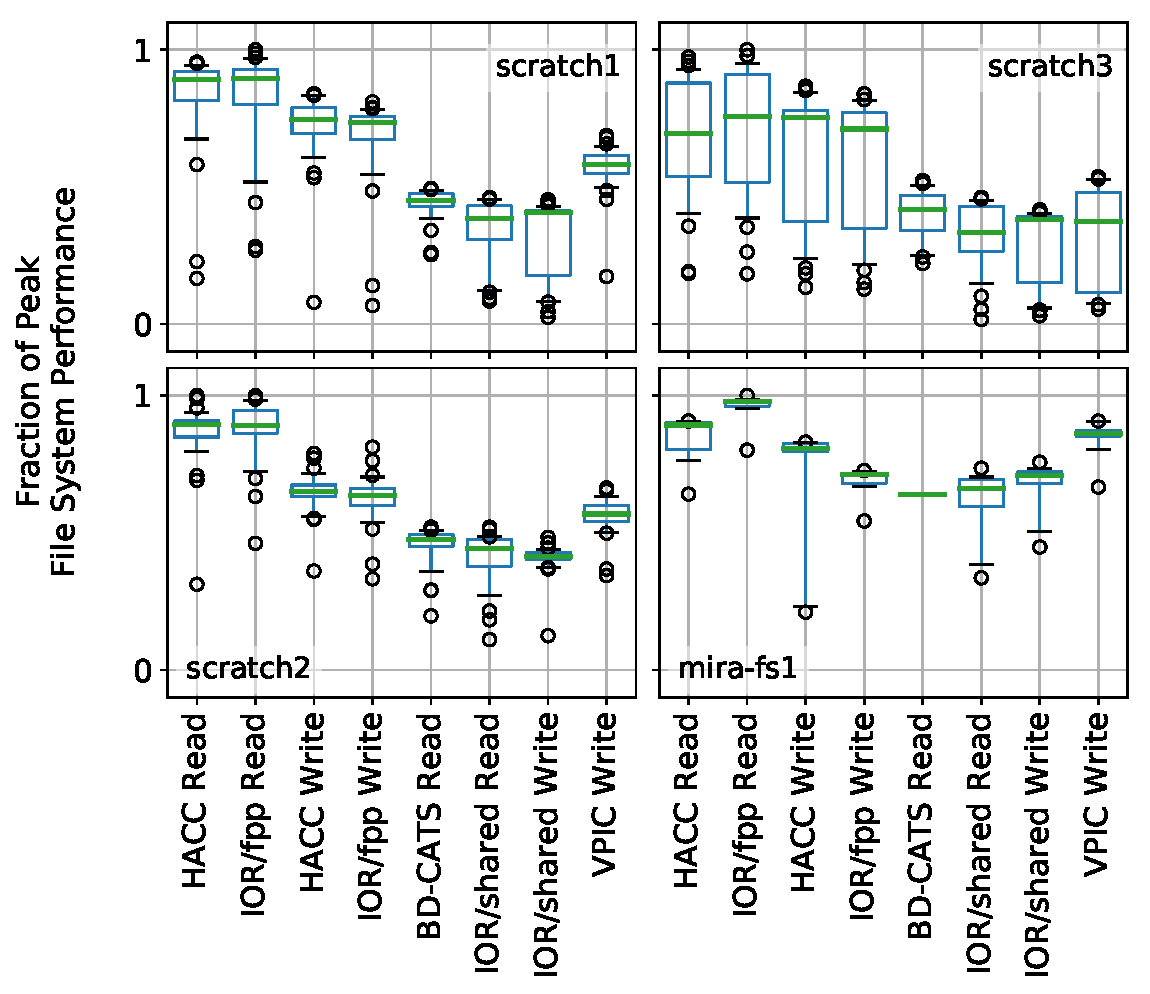
\includegraphics[width=1.0\columnwidth]{figs/perf-boxplots-per-fs.pdf}
    \caption{I/O performance for Edison (scratch1, scratch2, scratch3) and Mira (mira-fs1), normalized to the maximum performance of all tests performed on each file system.
    Each box reflects the distribution of an application workload and its read or write performance.
    Whiskers extend to the 5th and 95th percentiles.}
    \label{fig:perf-summary-boxplots-fs}
\vspace{-.2in}
\end{figure}

Such variation in peak file system performance caused by different I/O access patterns is well documented~\cite{Lofstead2010,Uselton2010,Xie2012}.
To focus solely on the variation caused by factors \emph{extrinsic} to each application, we then define the \emph{fraction of peak performance} as the performance of a job divided by the maximum performance observed for all jobs \emph{of the same I/O motif} as listed in Table \ref{tab:bench-config} and whether the job did reads or writes.
For example, the fraction peak performance for a HACC write test is only normalized to the maximum performance of all other HACC write tests on the same file system.
References to fraction peak performance are hereafter defined this way.

This fraction peak performance distribution, shown in Figure~\ref{fig:perf-summary-boxplots-motif}, reveals that the degree of performance variation \emph{within} each application also varies with each file system.
For example, the HACC write workload is susceptible to a long tail of performance degradation on mira-fs1 despite that file system's overall lower variation shown in Figure~\ref{fig:perf-summary-boxplots-fs}.
Similarly, all Edison file systems show a long tail of performance loss for the IOR/shared file read workload.
Edison's scratch3 also demonstrates very broad performance variation for the VPIC write workload, contrasting with the relatively narrow performance variation of this application on other systems.

\begin{figure}[t]
    \centering
    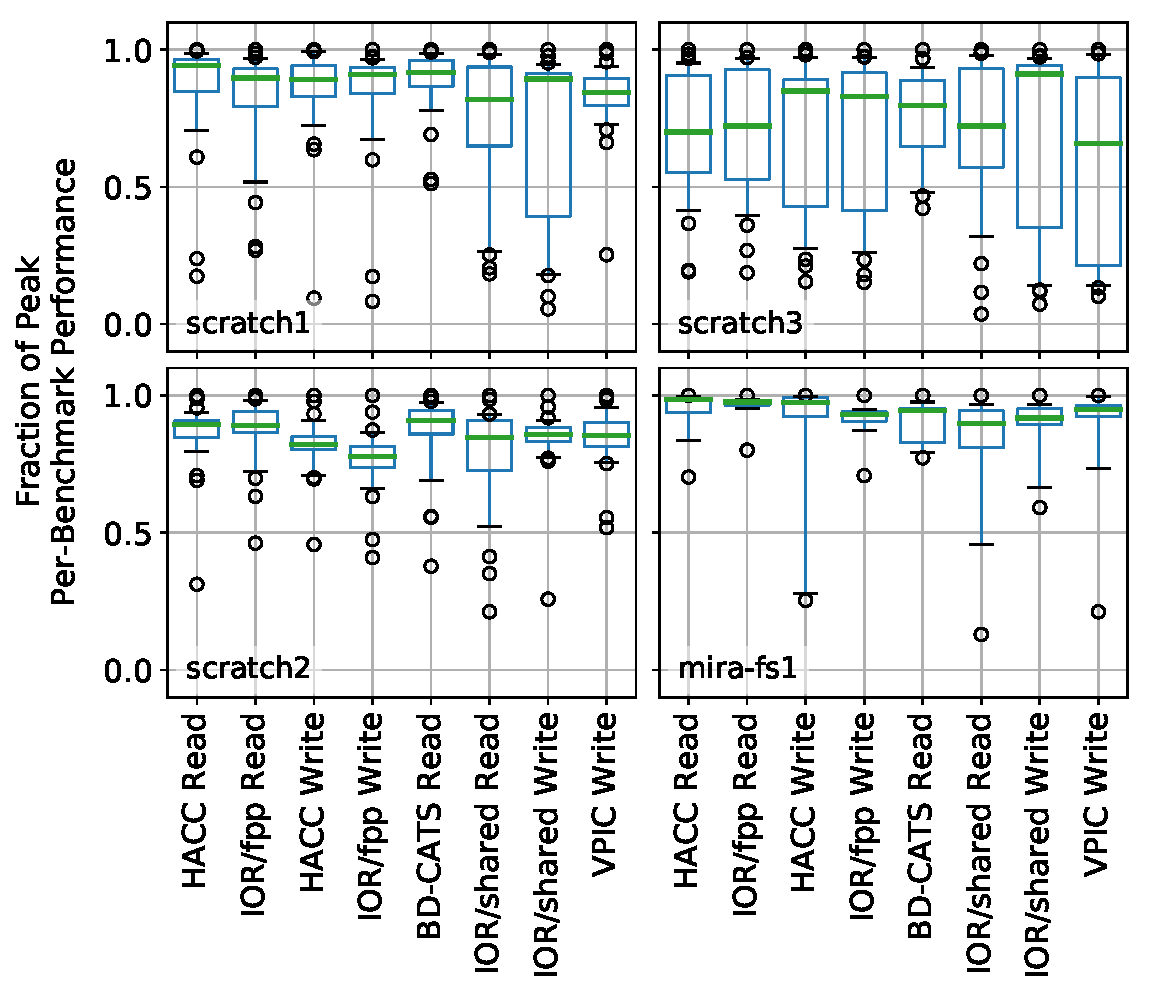
\includegraphics[width=1.0\columnwidth]{figs/perf-boxplots.pdf}
    \caption{I/O performance for all file systems tested grouped by test
    applications and read/write mode.  Whiskers represent the 5th and 95th
    percentiles.}
    \label{fig:perf-summary-boxplots-motif}
\vspace{-.2in}
\end{figure}

Thus, Figure \ref{fig:perf-summary-boxplots-motif} demonstrates that performance variability is the result of factors intrinsic to the application (e.g., I/O motif) \emph{and} factors intrinsic to the file system. 
Different I/O motifs result in different levels of performance \emph{and} variability.
Furthermore, these behaviors are not a function of the parallel file system software architecture either; all Edison file systems are Lustre-based, yet there is a marked difference in variability between scratch1/scratch2 and scratch3 shown in Figure~\ref{fig:perf-summary-boxplots-motif}.
Thus, these differences in performance variation must be a result of their different hardware configurations (discussed in Section \ref{sec:platforms}), their specific user workloads, or a combination of both.

%%%%%%%%%%%%%%%%%%%%%%%%%%%%%%%%%%%%%%%%%%%%%%%%%%%%%%%%%%%%%%%%%%%%%%%%%%%%%%%%
\subsection{Combined Application/Server Metrics} \label{sec:results/combining}
%%%%%%%%%%%%%%%%%%%%%%%%%%%%%%%%%%%%%%%%%%%%%%%%%%%%%%%%%%%%%%%%%%%%%%%%%%%%%%%%

To better understand how performance variation is caused by factors extrinsic to the application, we combine data from application-level analysis provided by Darshan with storage system traffic analysis provided by LMT (Edison) and ggiostat (Mira).
An intuitive source of performance loss would be from other jobs that are also consuming file system bandwidth, so to explore the effects of competing I/O traffic, we define the \emph{coverage factor} ($\mathit{CF}$) of a job $j$:

\begin{equation} \label{eq:cf}
    \mathit{CF}(j) = \frac{N_{\textup{bytes}}^{\textup{Darshan}}(j)}
    {\sum_{t,s}^{\textup{time,servers}}
    \left [ N_{\textup{bytes}}^{\textup{LMT,ggiostat}}(t,s) \right ] }
\end{equation}
%
where $N_{\textup{bytes}}^{\textup{Darshan}}$ is the number of bytes read and written by job $j$ according to its Darshan log, and $N_{\textup{bytes}}^{\textup{LMT,ggiostat}}$ is the number of bytes read and written to a parallel file system server $s$ during a 5-second time interval $t$.
The time interval over which the job ran ($\mathit{time}$) and the servers to which the job wrote ($\mathit{servers}$) are both taken from the job's Darshan log~\cite{snyder2016modular}.
% It should be noted that we can generalize this notion of the coverage factor to any metric for which we can distinguish the contribution of an individual job from the global system-level measurement, but for brevity in this work we focus our analysis on bandwidth coverage factor.

The coverage factor is a direct reflection of how much I/O traffic a job competed against in the underlying file systems.
$\mathit{CF} = 1.0$ when all of the server-side I/O was caused by job $j$, while $\mathit{CF} = 0.5$ indicates that only half of the server-side I/O was attributable to job $j$ while the other half came from other sources.
In practice, $\mathit{CF}$ can be slightly greater than $1.0$ as a result of two conditions:
a) when the storage system traffic monitoring (LMT/ggiostat) does not capture data from all servers during a polling interval, or
b) when clock skew between the compute nodes and the file system servers causes the Darshan log and LMT/ggiostat to have an inconsistent understanding of when I/O happened.
%%% GKL: Nick pointed out that the CF > 1.2 data we dropped are not noise, they are the component monitoring being completely broken.
In this study, such noise never resulted in $\mathit{CF} > 1.2$.
%To eliminate obviously erroneous data, we discard all test results where $\mathit{CF} > 1.2$ in the subsequent analysis.
% \todo{We should probably mention what \% of data this covers. It will be a likely question.}
%%% GKL: I don't want to admit to this unless a reviewer specifically asks.  The ratio is very high on Mira; 96 of the 214 measurements provided by Shane were dropped due to this  filter criterion

\begin{figure}[t]
    \centering
    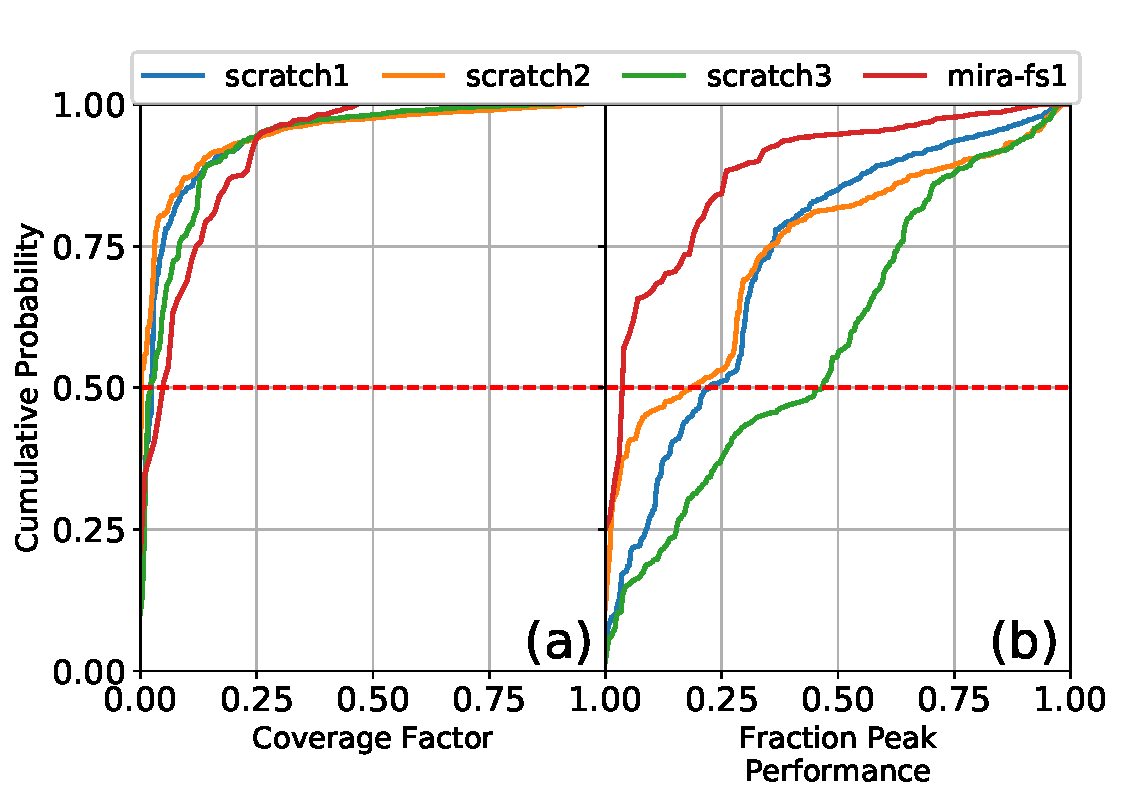
\includegraphics[width=\columnwidth]{figs/cdf-both.pdf}
    \caption{Cumulative distribution function of the coverage factor (a) and the    performance relative to the maximum throughput observed across each file system (b).
    The line demarcating 50\% probability corresponds to coverage factors of 0.88, 0.87, 0.84, and 0.94 and peak performance fractions of 0.89, 0.86, 0.78, and 0.95 on Edison scratch1-scratch3 and Mira, respectively.}
    \label{fig:cdfs}
\vspace{-.2in}
\end{figure}

%The distribution of coverage factors across all experiments run are shown in Figure~\ref{fig:cdfs}a which reveals that the majority of tests ($> 75\%$ on Edison and $> 80\%$ on Mira) have high coverage factors ($\mathit{CF} > 0.80$).
%This is consistent with the observation that I/O occurs in bursts~\cite{Carns2011,Liu2016}, and the probability of two bursts coinciding and causing contention for bandwidth (thereby reducing $\mathit{CF}$) is relatively low.
%In particular, Mira's $\mathit{CF}$ distribution is so narrow that over 50\% of tests effectively ran without bandwidth contention; $\mathit{CF} >= 0.99$ corresponds to the 40th percentile on that system.

The distribution of coverage factors across all experiments revealed that ($> 75\%$ on Edison and $> 80\%$ on Mira) have high coverage factors ($\mathit{CF} > 0.80$).
This is consistent with the observation that I/O occurs in bursts~\cite{Carns2011,Liu2016}, and the probability of two bursts coinciding and causing contention for bandwidth (thereby reducing $\mathit{CF}$) is relatively low.
In particular, Mira's $\mathit{CF}$ distribution is so narrow that over 50\% of tests effectively ran without bandwidth contention; $\mathit{CF} >= 0.99$ corresponds to the 40th percentile on that system.

Despite this low incidence of overlapping bursts, the distribution of performance relative to the peak observed bandwidth for each application such as shown in Figure~\ref{fig:perf-summary-boxplots-motif} is more broadly distributed.
Edison's scratch3 exemplifies this; 26\% of jobs on that file system got less than half of the peak performance (fraction peak performance $< 0.50$) despite only 5\% of jobs showing $\mathit{CF} < 0.50$.  This indicates that the coverage factor (and therefore server-side I/O bandwidth) is not the only contributor to sub-optimal performance.
This finding is consistent with previous work that found Lustre file system performance to be constrained by both bandwidth \emph{and} I/O operation (IOP) rate~\cite{Uselton2013}.

% \begin{figure}[t]
%     \centering
%     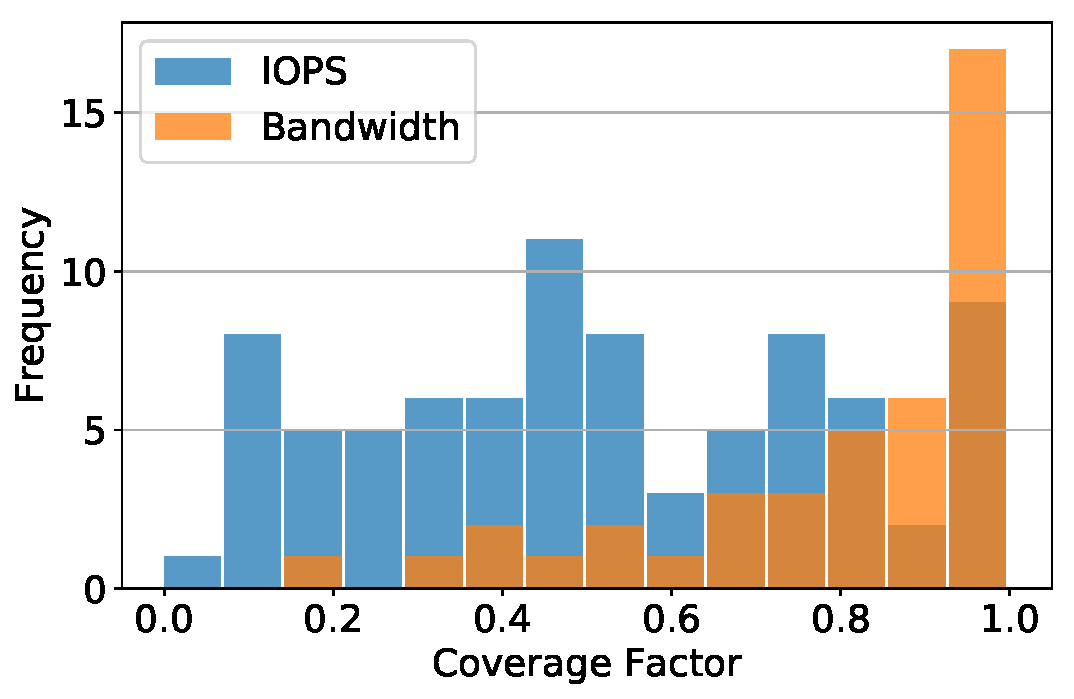
\includegraphics[width=\columnwidth]{figs/hist-cf-bw-and-ops.pdf}
%     \caption{Distribution of the coverage factor for both bandwidth ($\textit{CF}_{\textup{bandwidth}}$) and read/write operations ($\textit{CF}_{\textup{iops}}$) for Mira.
%     }
%     \label{fig:hist-cf-mira}
% \vspace{-.2in}
% \end{figure}
% 
% We can generalize this notion of the coverage factor to any metric for which we can distinguish the contribution of an individual job from the global system-level measurement.
% However, these alternative coverage factor metrics are not likely to correlate well with performance unless the job of interest is making a meaningful contribution to the system-wide load.
% For example, the coverage factor for IOPs can be expressed as the fraction of read and write operations extracted from a job's Darshan log to the total read and write operations logged by ggiostat.  The distribution of this $\textit{CF}_\textit{IOPs}$ metric is shown alongside the bandwidth coverage factor, $\textit{CF}_\textit{BW}$, in  Figure \ref{fig:hist-cf-mira}.
% This figure suggests that the TOKIO-ABC tests likely do not contribute a significant IOPs load Mira;
% the relatively flat distribution of $\textit{CF}_\textit{IOPs}$ is likely a reflection of the background IOPs load which is not significantly perturbed when TOKIO-ABC jobs are running. \todo{is there is a clearer way to state the previous sentence?}
% 

%%%%%%%%%%%%%%%%%%%%%%%%%%%%%%%%%%%%%%%%%%%%%%%%%%%%%%%%%%%%%%%%%%%%%%%%%%%%%%%%
\subsection{Correlating Performance Metrics} \label{sec:results/correlating}
%%%%%%%%%%%%%%%%%%%%%%%%%%%%%%%%%%%%%%%%%%%%%%%%%%%%%%%%%%%%%%%%%%%%%%%%%%%%%%%%

Although bandwidth is the most intuitive initial metric for application and server
correlation,  
%Our choice to define our correlation parameter according to application performance and server-side bandwidth and IOPs was motivated by a broad body of literature and an intuitive assumption that competition for bandwidth and IOPs affect performance the most dramatically.
%the TOKIO framework is generalized to draw data from any resource that can be indexed on a per-job or time series basis.
%Thus,
we can calculate correlations of other metrics with job I/O performance to objectively determine which of these are the likely culprits causing poor application performance.
To this end, we calculated the Pearson correlation coefficient between each job's fraction of peak performance (as defined in Section \ref{sec:results/overview}) with a wide range of metrics collected on Edison and Mira.
While many of these metrics are not expected to be normally distributed~\cite{Kim2010}, Pearson correlation coefficients are applied here to compare the directions and relative strengths of the relationships between each metric we analyzed.
In this sense, we find that this correlation coefficient is a suitable qualitative indicator of general trends and confidences in correlation.
A summary of some of the interesting correlations (and lack of correlations) are presented in Figure \ref{fig:correlation-table} and highlight several interesting findings:

\begin{figure}[t]
    \centering
    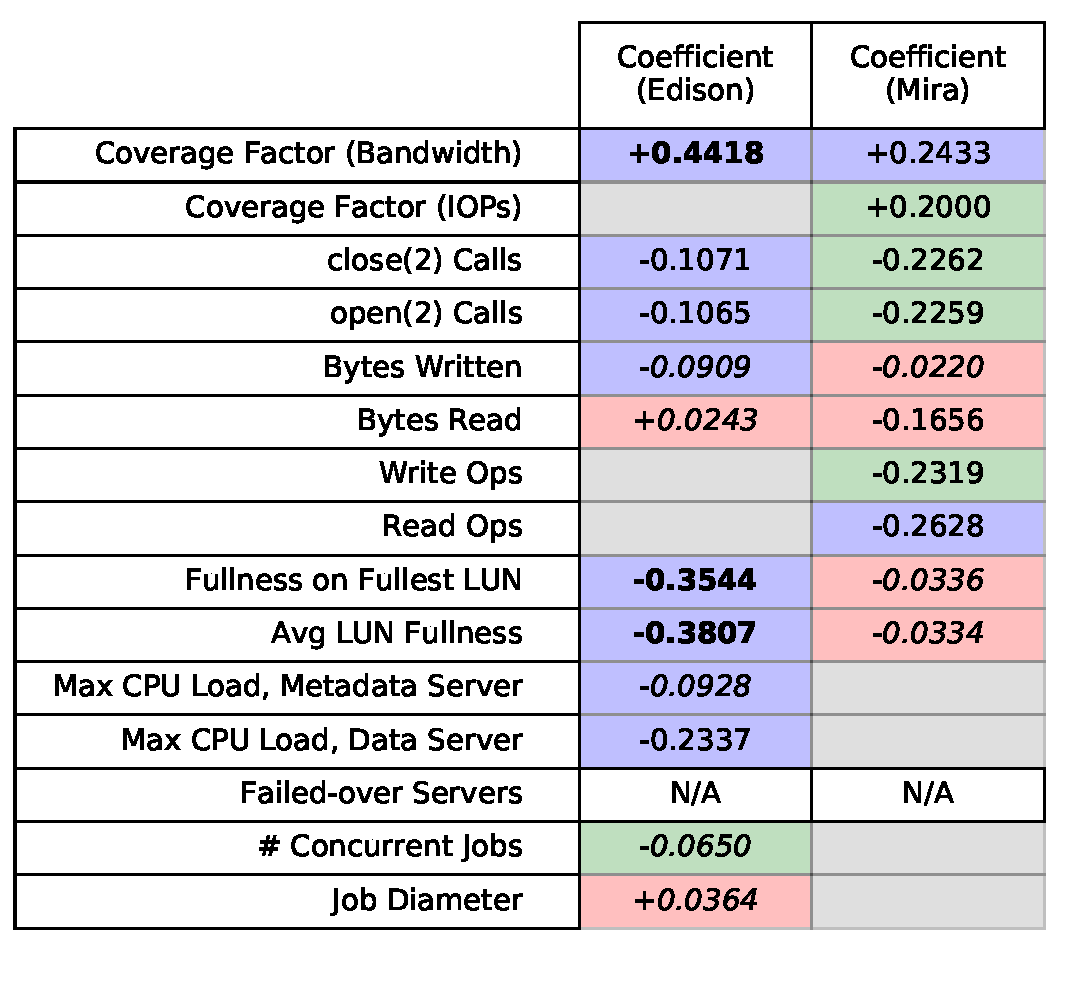
\includegraphics[width=\columnwidth]{figs/correlation_table.pdf}
    \caption{Correlation coefficients between fraction of peak performance measured for each I/O motif and a variety of server-side measurements and metrics.
    Box color indicates confidence; correlations with p-values $< 0.01$ are blue; p-values $< 0.05$ are green, and p-values $>= 0.05$ are red (and signify lack of correlation).
    Similarly, \textbf{bolded} values signify moderate correlation ($|r| > 0.30$), and \textit{italicized} values signify weak correlation ($|r| < 0.10$).
    The "\% Servers Failed Over" metric is not applicable because no
    changes in server failover state were
    observed during this study.
    }
    \label{fig:correlation-table}
\vspace{-.2in}
\end{figure}

\begin{itemize}[leftmargin=*]

\item As assumed in the previous sections, the coverage factors correlate with performance on all file systems, indicating that contending for file system I/O is a moderate contributor to performance loss.
The strength of this correlation on Mira was lower than Edison because the absolute performance of our tests on Mira were bound by the bandwidth of the exclusively allocated I/O nodes, leaving bandwidth headroom on the NSD servers for other jobs.
Mira's file system also demonstrated moderate sensitivity to contention for
IOPs, a metric that we were unable to collect on Edison in this study.
%Lustre IOPs were not collected for this study, so no comparison can be made to Edison.

\item Mira's performance correlates negatively with higher rates of \texttt{open(2)}/\texttt{close(2)} calls than Lustre.
Given that Mira's file system serves metadata from the same physical servers as data, this relationship is reasonable.
By comparison, Edison's file systems each have their own discrete metadata servers that are specifically designed to decouple bulk data transfer performance from metadata operations.

\item The fullness of each storage device (LUN on Mira and OST on Edison) has markedly different behavior between Edison and Mira.
While Mira's performance is uncorrelated with device capacity, Edison performance degrades as free space on OSTs is depleted.
This type of behavior is a known characteristic of the Lustre file system and has been observed on deployments at other HPC centers~\cite{oral2014best}, as well.
%This is a documented behavior of Lustre file systems~\cite{oral2014best}.

\item Perhaps contrary to historic intuition, I/O performance shows minimal correlation with the number of other jobs running concurrently.
The lack of correlation with concurrent job count is consistent with our finding that I/O remains highly bursty; a large number of small jobs are highly unlikely to burst simultaneously, and each small job is not individually capable of significantly impacting our tests' coverage factors.

\item Similarly, the job diameter (a measurement of how spread out a job is across the compute fabric) has no discernible correlation with I/O performance on Edison.
Since the low-diameter dragonfly topology of Edison is designed
to reduce the performance impact of job topology, this is consistent with
expectation.  Job diameter is not shown for Mira because it utilizes a dense
torus partition for each job.

\end{itemize}

We collected additional system-specific measurements that did not correlate significantly to performance.
However it is important to underscore the fact that this demonstration was not intended to be exhaustive, and the correlations and p-values for the Edison system are likely diminished by the fact that data for all three Edison file systems were combined for this analysis.

%%%%%%%%%%%%%%%%%%%%%%%%%%%%%%%%%%%%%%%%%%%%%%%%%%%%%%%%%%%%%%%%%%%%%%%%%%%%%%%%
\section{Job-Level Analysis} \label{sec:results/umami}
%%%%%%%%%%%%%%%%%%%%%%%%%%%%%%%%%%%%%%%%%%%%%%%%%%%%%%%%%%%%%%%%%%%%%%%%%%%%%%%%

This holistic I/O analysis is not only useful to understand broad system behavior as illustrated in Section~\ref{sec:results}, but also to understand the factors that contribute to the performance of individual application executions.
The system-level analysis can be integrated with ongoing I/O instrumentation to describe
where on the spectrum of normalcy a job's I/O behavior fell relative to
jobs with similar motifs and which metrics are the most promising starting point for
investigation based on historic correlation.

\begin{figure}[t]
    \centering
    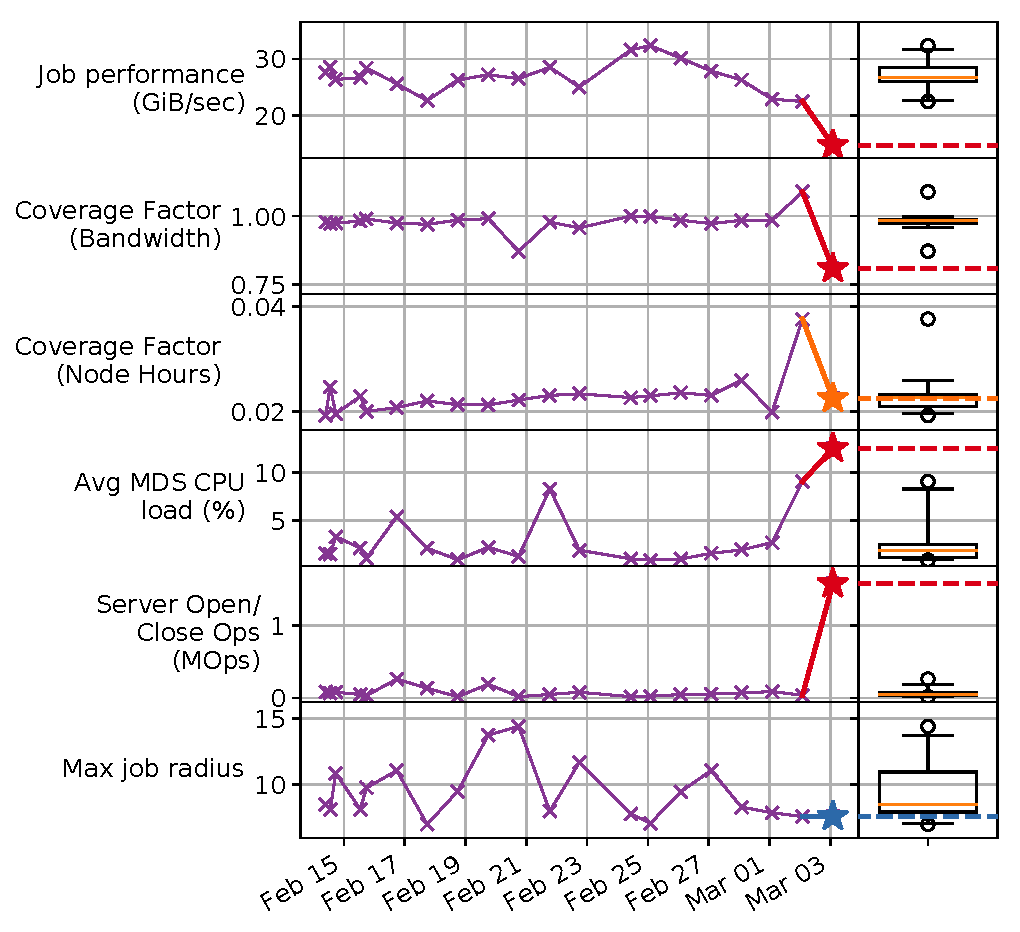
\includegraphics[width=1.0\columnwidth]{figs/umami-scratch2-hacc-write.pdf}
    \caption{UMAMI demonstrating the \emph{file system climate} of HACC write workloads on the Edison scratch2 file system compared to a most recent run, which showed highly unusual \emph{file system weather}.
    The left panes show the measurements from previous runs of the same motif, and the box plots in the right panes summarize the distribution of these metrics.
    The star denotes the metrics for the job of interest and is colored according to the quartile in which it falls (red being the worst quartile and blue the best).
    Box plot whiskers extend to the 5th and 95th percentiles, with outliers being denoted as circles.}
    \label{fig:umami-scratch2-hacc-write}
\vspace{-.2in}
\end{figure}

To concisely visualize all of this information, we present a Unified Measurements And Metrics Interface (UMAMI) as a tool to quickly determine how a job of interest's performance compares to similar I/O workloads in the past.
UMAMI, demonstrated in Figure \ref{fig:umami-scratch2-hacc-write} and detailed in the following sections, presents historic measurements (the I/O climate) and summarizes each metric's distribution in an accompanying box plot.
These time series plots terminate with the measurements relevant to the job of interest, thereby describing the I/O weather at the time that job ran.
By overlaying this weather on the climate as dashed lines in the box plots, UMAMI provides a quick visualization of how each metric's contribution to weather compared to the statistical distribution of past weather conditions.
With this conceptualization of a file system's weather and its overall climate, a user can differentiate between a long-term performance problem and a statistically rare event analogous to an extreme weather event.

% In the following sections, we illustrate how UMAMI can be applied to the problem of diagnosing poor performance of individual jobs in three case studies.

\subsection{Case Study: I/O Contention}

The specific UMAMI example shown in Figure \ref{fig:umami-scratch2-hacc-write} represents a HACC write test which took place on March 3.
This particular job showed abnormally low performance as evidenced by the "Job performance (GiB/sec)" measurement and its value relative to previous instances of this type of job.
This abnormally poor job performance was accompanied by an unusually low coverage factor and high metadata load, and these unfavorable conditions are highlighted as red dashed lines in the box plots that denote their place in the least-favorable quartile of past measurements.
The metrics corresponding to blue dashed lines fell into the most favorable quartile for this problematic job, but as discussed in Section \ref{sec:results/correlating}, they have no history of correlation with performance.
Thus, we can quickly attribute the poor performance of this HACC job to an I/O load extrinsic to this job which was competing for both bandwidth on the data servers and metadata resources on the metadata server.

\subsection{Case Study: Metadata Load}

Figure \ref{fig:umami-mira-fs1-vpic-write} represents a VPIC write workload
that showed poor performance on Mira.
Its coverage factor is within normal parameters (orange lines in each metric's box plot signifies a value in the second quartile) indicating low bandwidth contention.
Although the IOPS coverage factor is also abnormally low, previous conditions have been worse despite a lack of dramatic performance loss (e.g., on March 7).
The only metric that shows a unique, undesirable value is the number of \texttt{readdir(3)} operations handled by the file system.
This is indicative of an expansive file system traversal that was being performed at the same time as the job execution.
% The \emph{readdir(3)} metric was demonstrated to correlate moderately negatively with performance in Figure \ref{fig:correlation-table}.

\begin{figure}[t]
    \centering
    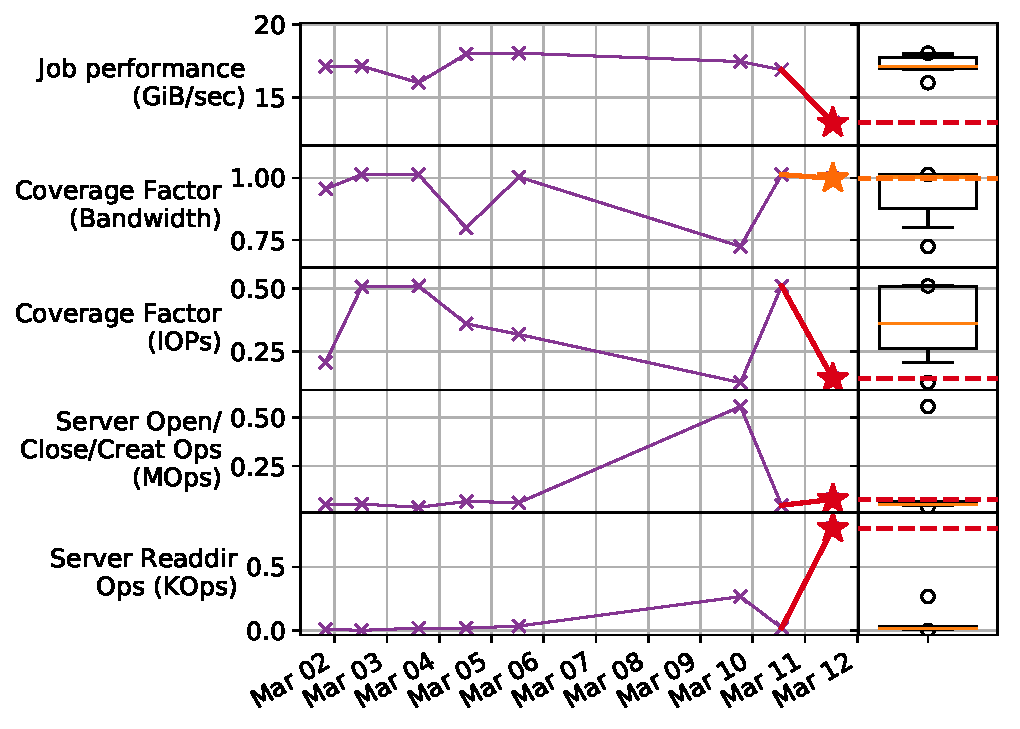
\includegraphics[width=1.0\columnwidth]{figs/umami-mira-fs1-vpic-write.pdf}
    \caption{UMAMI demonstrating the climate surrounding VPIC-IO write workloads on Mira compared to a most recent run, which showed highly unusual weather in the form of an excess of \texttt{readdir(3)} calls.
    Significance of each pane and its contents are the same as explained in Figure \ref{fig:umami-scratch2-hacc-write}.}
    \label{fig:umami-mira-fs1-vpic-write}
\vspace{-.2in}
\end{figure}

%%%%%%%%%%%%%%%%%%%%%%%%%%%%%%%%%%%%%%%%%%%%%%%%%%%%%%%%%%%%%%%%%%%%%%%%%%%%%%%%
\subsection{Case Study: Storage Capacity}
%%%%%%%%%%%%%%%%%%%%%%%%%%%%%%%%%%%%%%%%%%%%%%%%%%%%%%%%%%%%%%%%%%%%%%%%%%%%%%%%

This holistic approach is also able to identify longer-term performance issues that progressively degraded write performance.
Figure \ref{fig:umami-scratch3-hacc-write-long-term} shows the UMAMI view of such an event on Edison's scratch3 file system where coverage factors were not highly abnormal despite an ongoing $2\times$ slowdown over the normal 50 GiB/sec.
The magnitude of performance loss followed the highest CPU load observed across all of the Lustre OSSes almost exactly, and this period coincided also with the scratch3 file system reaching critical levels of fullness.
Although such correlations cannot define causative relationships, these conditions indicated a relationship between critically full storage devices and CPU load (e.g., an increasing cost of scavenging empty blocks) that impacts application performance, consistent with our understanding of how Lustre performance degrades as OSTs fill~\cite{oral2014best}.
 
\begin{figure}[t]
    \centering
    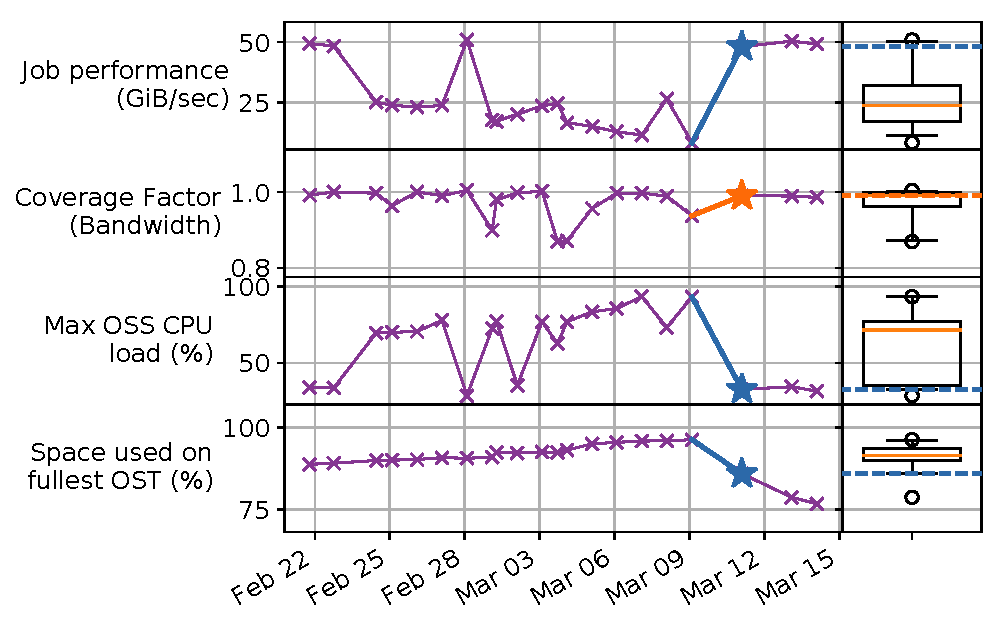
\includegraphics[width=1.0\columnwidth]{figs/umami-scratch3-hacc-write-long-term.pdf}
    \caption{UMAMI of HACC write performance on Edison's scratch3 file system showing a longer-term period of performance degradation that was associated with unusually high OSS CPU load.
    Significance of each pane and its contents are the same as explained in Figure \ref{fig:umami-scratch2-hacc-write}.}
    \label{fig:umami-scratch3-hacc-write-long-term}
\vspace{-.2in}
\end{figure}


\section{Related work} \label{sec:related}

Several recent studies have explored how to combine
and analyze multiple sources of I/O monitoring information.
Kunkel et al. developed the Scalable I/O for Extreme Performance
(SIOX)~\cite{Kunkel:2014:SAC:2769884.2769901}, which aggregates
information from multiple layers of the I/O stack into a global database
with plugins for automatic optimization.  It relies on instrumented
versions of application libraries to collect metrics.  Agelastos et al.
developed the Lightweight Distributed Metric Service (LDMS)~\cite{7013000}
for scalable collection of compute node metrics. The LDMS metrics include
client-side I/O counters that could be integrated into TOKIO.  Liu et al. applied in-depth
analysis to server-side I/O logs to deduce application-level I/O patterns
and make scheduling recommendations~\cite{Liu2016}.

Other recent studies have explored how to quantify and combat various
types of I/O performance variance.  Lofstead et al. observed that
variability can can be caused not only by external interference, but also
internal interference within an application~\cite{Lofstead2010}.
They proposed an adaptive I/O strategy that coordinates I/O activity
within an application.  Dorier et al. proposed a middleware mechanism
for coordinating I/O activity across applications to manage external
interference~\cite{dorier2014calciom}.  Yildiz et al. performed a
systematic study of I/O interference in a controlled testbed environment,
and found that variance often arose from poor flow control in the I/O
path~\cite{Yildiz2016}.  Carns et al. reported I/O performance variability
for seven frequently repeated production jobs during a two month study
of the Intrepid Blue Gene/P system~\cite{carns2011understanding}.
Their results suggested that some access patterns are more susceptible
to variability that others, but the root cause of that variability was
not identified.

Our work builds on these previous studies by introducing a framework that
integrates multiple existing best-in-class characterization tools into a
general analysis framework that can be adapted to any platform.

%for each
%component in a manner that can be rapidly adapted to different platforms.  We
%invision this as a way to rapidly provide feedback and contextual information to
%users as they execute their applications.

% Andrew Uselton's work on understanding I/O performance in terms of ensembles of
% bursts might be relevant\cite{Uselton2010}, but his method requires heavyweight
% I/O tracing to determine the statistical distribution of I/O bursts during an
% application execution and, as such, as better suited to characterizing the
% behavior of a specific file system as a one-time activity.

% A long time ago, David Skinner and Bill Kramer wrote a paper that characterized
% sources of performance variation~\cite{Skinner2005}, but it didn't really talk
% about I/O in a very meaningful way.

% More recently Xie et al also characterized I/O problems at Oak
% Ridge\cite{Xie2012} using IOR and quantified the effects of stripe counts,
% straggling writers, and shared-file I/O to target areas where middleware can
% optimize I/O for applications.

% Is any of the BeeGFS stuff (dynamically provisioning file systems) relevant to
% interference isolation?


\section{Conclusions and Future Work} \label{sec:conclusions}

% Attempting to understand I/O behavior on modern-day HPC systems is a daunting task, due in large part to the increasingly complex and hierarchical nature of the underlying I/O subsystem.
Understanding I/O behavior on modern-day HPC systems is a daunting task, due in large part to the increasingly complex and hierarchical nature of the underlying I/O subsystem.
% In this work we have presented TOKIO, a powerful framework providing holistic instrumentation and analysis of HPC I/O subsystem behavior by collecting and integrating data from numerous components throughout the system.
To address this growing complexity, we have presented TOKIO, a powerful framework for integrating data from numerous components throughout the HPC I/O subsystem to provide holistic analysis of I/O behavior.
% We have leveraged the TOKIO framework to investigate I/O subsystem behavior on two leadership-class HPC systems, with each system subjected to daily I/O performance regression benchmarking over a 1-month period.
We have applied the TOKIO framework to investigate I/O performance variation on two large-scale HPC systems, with each system subjected to daily I/O performance regression benchmarking over a month-long period.
We used the data generated by this experiment to first characterize the I/O \emph{climate} on each system, and then to detect and investigate particular instances of abnormal I/O \emph{weather}.

By integrating a range of distinct, normalized monitoring metrics into the
TOKIO-UMAMI tool, we have provided a coherent foundation for simplified
characterization of HPC I/O behavior across different platforms, thereby
enabling previously impractical comparative studies and sharing of analysis
methods. 
In this study we applied the TOKIO framework to show that I/O performance is affected by both intrinsic application characteristics and extrinsic storage system factors. Contention with other I/O workloads for storage system bandwidth is not the only factor that affects I/O performance; %we observed numerous instances of jobs that had uninhibited access to storage system resources that still exhibited poor I/O performance
we highlight cases  where namespace contention and storage capacity both dramatically impacted performance.
%and a moderate inverse correlation between performance and extrinsic read/write operations
We also show that there is no single monitoring metric that predicts I/O performance
universally across HPC platforms; the most highly correlated metrics depend
on system architecture, configuration parameters, workload characteristics,
and system health.

In future work we will incorporate additional sources of I/O subsystem
instrumentation, explore to what degree the TOKIO capability can be made
available to end users, apply more in-depth statistical analysis to data
as it is archived over time, and investigate alternative groupings of
metrics to identify combinations of applications that produce
adversarial I/O load.

%We were also able to use TOKIO for providing in-depth analysis of jobs exhibiting particularly poor I/O performance to attempt to uncover potential root causes.
%We developed the TOKIO-UMAMI analysis tool to help diagnose I/O performance problems by contextualizing the historical trends of pertinent I/O metrics with the values observed for a specific job of interest.

%This study explored only one of the potential applications of TOKIO though.  Looking forward, it is possible to group historic data around server-side traffic patterns rather than application I/O motifs to identify collections of applications that, when run together, result in an uncommonly adversarial I/O load.  This could advise coscheduling to optimize performance.  In addition, the grouping process itself can be automated with clustering or other statistical techniques to explore emergent I/O behavior in an unbiased fashion.

%%% GKL: I would really like to propose plugging Xiaosong Ma's clustering-based burst classification into this so that TOKIO-UMAMI can automatically figure out which jobs should define climate.  Not sure where it will fit though...
% Capturing an historic record of a file system's climate for a particular workload is not always straightforward, and at present, users will have to self-identify jobs and Darshan logs that should be used to build this historic record.
% Alternatively, UMAMI can be seeded with data from baseline performance tests, as was done in this study, provided that the user's I/O motif is sufficiently similar to one of the baseline tests' motifs.
% This can be automated to a large degree though; the simplest approach is to scan Darshan logs for similar I/O transaction size distributions as seeds.
% Recently, Liu et al have also demonstrated combining resource manager logs and server-side I/O logs to identify a series of I/O bursts with specific jobs using a density-based clustering method~\cite{Liu2016}.
% We believe that adapting this clustering-based classification approach with TOKIO-UMAMI should be a straightforward approach to building an I/O climate record for any arbitrary job.

% \todo{It would be great if there were some tangible artifacts from this work.
% Possible examples:}
% \begin{itemize}
% \item open repo for benchmark configs and cron jobs so others can replicate
% performance regression testing
% \item anonymized data collected in study
% \item new data collection tools (LMT monitoring, Lustre failover monitoring,
% mmpmon monitoring, etc.)
% \end{itemize}

%%% GKL: I lament the removal of these high-level findings :(
%%% they seem highly quotable, and I feel like we might be giving up future citations by not explicitly stating this stuff.
% Overall, instances of abnormally poor I/O performance on Mira were most often attributable to equally abnormal coverage factors (indicating bandwidth contention) or high metadata rates (opens/closes and readdirs).
% Of all \todo{UPDATE}92 tests run on this file system, only one case of performance falling in the first quartile was not accompanied by one of these server-side contention conditions.
% The most common sources of performance loss on Edison were more difficult to neatly categorize because server-side IOPS were not measured explicitly.
% In those cases where performance was poor despite a high coverage factor, many secondary indicators of high IOPS load (such as high data server CPU load and high metadata rates) were observed.

% Qualitatively, the highly variable I/O workload and "I/O weather" conditions across the Edison file systems obfuscate a straightforward analysis of all of the sources of performance variation on its file systems.
% Over the course of this study, we found that the TOKIO framework often exposed variation resulting from the confluence of several factors that only correlate weakly with performance when examined independently.
% Thus, TOKIO requires some amount of expert knowledge to confidently determine the root cause of I/O problems on file systems that are subject to large amounts of incoherent or otherwise noisy I/O.
% That said, presenting the historic correlations between performance and each variable through UMAMI does dramatically reduce the exploration space in this effort.

%%% GKL: this might be appropriate if we want to include future outlook or other use cases
% Finally, although we applied TOKIO and UMAMI to build I/O climate histories specific to applications based on Darshan logs, it is equally possible to group historic data around similar periods of server-side traffic.
% For example, TOKIO can be used to identify collections of applications that, when run together, result in an uncommonly adversarial I/O load or, conversely, surprisingly good performance.
% From this, it is easy to envision an opportunity to inform job scheduling to avoid I/O contention between two frequently conflicting applications.


% \section{TEMPORARY: TECHNICAL TASKS}
% 
% Assumption: assignments here and in preceding text are tentative, and really
% just guess at someone who can keep tabs on that activity.  Can re-assign,
% delegate, pull in more people, etc.
% 
% \begin{itemize}
%     \item \textcolor{red}{ALL}: Begin analyzing TOKIO-ABC benchmark results and
%     and think about how we want to correlate this with GPFS/Lustre monitoring
%     data. Are there specific jobs or timeframes that we want to zoom in on
%     to better understand anomalous behavior? Are there I/O trends that we
%     can observe on specific systems or even across systems that would be
%     interesting to the reader? This is where we want to showcase the utility
%     of this framework, so we will need to find something interesting to demonstrate
%     here to convince the reader. 
% 
%     \item \textcolor{red}{ALL}: begin filling in paper intro, background,
%     methodology, system/benchmark descriptions, results, etc.
% 
%     \item \textcolor{red}{SHANE}: round up MMPMON data for a 2-week period
%     of TOKIO-ABC runs on Mira.
% 
%     \item \textcolor{red}{GLENN}: round up LMT data for a 2-week period of
%     TOKIO-ABC runs on Edison.
% 
%     \item \textcolor{red}{WILLIAM}: look at MMPMON data to determine how
%     IOMiner can be extended to analyze GPFS data. 
% \end{itemize}
% 
% Timeline:
% \begin{itemize}
%     \item \textcolor{red}{SC abstracts due March 20, 2017}
%     \item \textcolor{red}{SC full submissions due March 27, 2017}
%     \item Time to get moving!
% \end{itemize}

\bibliographystyle{ACM-Reference-Format}
\bibliography{REFERENCES}

\appendix

\subsection{Artifact Description} \label{sec:appendix/artifacts}

Consider adding material here per guidance at
\url{http://sc17.supercomputing.org/2017/02/07/submitting-a-technical-paper-to-sc17-participate-in-the-sc17-reproducibility-initiative/}.

\subsubsection{Abstract}

\subsubsection{Description}

\subsubsection{Meta Information}

\paragraph{Obtaining Software}

\paragraph{Hardware Dependencies}

\paragraph{Software Dependencies}

\paragraph{Datasets}

\subsubsection{Installation}

\subsubsection{Experiment Workflow}

\subsubsection{Evaluation and Expected Result}

\subsubsection{Experiment Customization}

\subsubsection{Notes}


\subsection{Computational Results Analysis} \label{sec:appendix/analysis}

Some types of additional diagnostics could be:
\begin{enumerate}
\item validation of the timers (time something with a known execution time, determine the precision and statistical variability of the timer).
\item Confirm results for a manufactured solution.
\item Test the analytics of the problem, e.g., generate a problem with known spectral properties and test its behavior.
\end{enumerate}



\end{document}
